\documentclass[oneside]{caesar_book}

%%%%%%%%%%%%%%%%%%%    PACKAGES    %%%%%%%%%%%%%%%%%%%
%% Font
\usepackage{fontspec}
\setmainfont{TexGyrePagella}

%% Languages
\usepackage{polyglossia}
	\setdefaultlanguage[variant=british]{english}

%% Author affiliation
\usepackage{authblk}

%% Figures...
% ...graphics
\usepackage[luatex]{graphicx}

\usepackage[font = small]{caption}
\usepackage{subcaption}
	\captionsetup{subrefformat=parens}
	% \captionsetup[subfigure]{skip=-30pt} % aboveskip=-30pt,belowskip=-2pt,

% ...Colours
\usepackage{xcolor}
	\definecolor{egyptRed}{HTML}{DD5129}
	\definecolor{egyptBlue}{HTML}{0F7BA2}
	\definecolor{egyptGreen}{HTML}{43B284}
	\definecolor{egyptYellow}{HTML}{FAB255}
	\definecolor{lightGrey}{HTML}{CCCCCC}

% ...TikZ coding
\usepackage{tikz}
	\usetikzlibrary{arrows.meta}
	\tikzset{arrow/.style = {> = {Latex[length = 1.2mm]}}}
	\usetikzlibrary{positioning}
	\usetikzlibrary{calc}
	\usetikzlibrary{fit}
	\usetikzlibrary{backgrounds} % Can be useful for debugging, i.e. check the frame of a tikz picutre. For this \begin{tikzpicture}[framed]

% Define database node
\makeatletter
	\tikzset{
		database/.style={
			path picture={
			\draw[fill = egyptYellow] (0, 1.5*\database@segmentheight) circle [x radius=\database@radius,
			y radius=\database@aspectratio*\database@radius];
			\draw (-\database@radius, 0.5*\database@segmentheight) arc [start angle=180,end angle=360,x radius=\database@radius,
			y radius=\database@aspectratio*\database@radius];
			\draw (-\database@radius,-0.5*\database@segmentheight) arc [start angle=180,end angle=360,x radius=\database@radius,
			y radius=\database@aspectratio*\database@radius];
			\draw (-\database@radius,1.5*\database@segmentheight) -- ++(0,-3*\database@segmentheight) arc [start angle=180,end angle=360,
			x radius=\database@radius, y radius=\database@aspectratio*\database@radius] -- ++(0,3*\database@segmentheight);
			},
			minimum width=2*\database@radius + \pgflinewidth,
			minimum height=3*\database@segmentheight + 2*\database@aspectratio*\database@radius + \pgflinewidth,
		},
		database segment height/.store in=\database@segmentheight,
		database radius/.store in=\database@radius,
		database aspect ratio/.store in=\database@aspectratio,
		database segment height=0.1cm,
		database radius=0.25cm,
		database aspect ratio=0.35,
	}
\makeatother

%% Links
\usepackage{url}
\usepackage[luatex, colorlinks=true, linkcolor=egyptBlue, urlcolor=egyptRed, citecolor=egyptGreen]{hyperref}

%% Bibliography
\usepackage{csquotes}
\usepackage[backend=biber,style=philosophy-classic]{biblatex}
\addbibresource{./centralised_bibliography/references.bib}



\usepackage{amsmath}
\usepackage{siunitx}

\usepackage{booktabs}



% Information about the book
% to be put on the title page
\title{Technical note on total and bole volumes to the Conseil Scientifique et Technique de l'IGN}

\author{Amaël Le Squin, Florence Gohon}

\publisher{}

%----------------------------------------------------------------------------------------
%	NEW COMMANDS
%----------------------------------------------------------------------------------------

\newcommand{\NFI}{NFI}
\newcommand{\ie}{\textit{i.e., }}

\begin{document}
% no page numbering in front matter
\frontmatter
% generate the title page
\maketitlepage
% show the table of contents
\tableofcontents
% start to number the pages
\mainmatter

\chapter{Context\label{chap::context}}

The French National Forest Inventory (\NFI) publishes statistics annually, such as basal area or wood resources, on both private and public forest. These statistics are derived from a sampling scheme in which about \num{6000} new plots are surveyed each year, along with \num{6000} plots that were first visited five years earlier. The published statistics are calculated using a moving five-year average; for instance, the published results for 2024 are based on campaigns spanning from 2020 to 2024. \\

Initially designed to assess forest area and produce estimates of standing timber stock, the French \NFI{} is gradually evolving into more comprehensive tools for forest monitoring, incorporating a variety of indicators. Among this new information, the estimation of forest biomass and carbon is crucial, as it makes it possible to monitor biomass production and its use by different sectors, to estimate the contribution of forests to mitigating the effects of climate change as part of climate commitments monitoring (Citepa), and to develop forest strategies adapted to contemporary environmental and societal challenges \parencite{Commission2018}. \\

% Check \sidecite, and maybe tweak it to put only the author and title in the margin

The European Union developed a \href{https://eur-lex.europa.eu/legal-content/EN/TXT/?uri=CELEX:52021DC0572}{New EU Forest Strategy for 2030} as part of the plan to adapt to and fight against climate change and make Europe a climate neutral continent by 2050. This strategy relies on improved monitoring of European forests to better understand their condition and respond accordingly. Specifically, it calls for assessing carbon sequestration in forests to evaluate whether or not Eu\-ro\-pe reached carbon neutrality. One bottleneck is the harmonisation of the forest monitoring methods between European member states, if not within them. The \href{https://pathfinder-heu.eu/#top}{PathFinder project} supports member states in implementing a European Forest Monitoring System in order to standardise or harmonise forest data collection and reporting across the EU. This prompted the French \NFI{} to update its methods for assessing forest carbon storage. \\

Three steps are necessary to estimate carbon storage from field data (see Fig. \ref{fig::scheme}): (\textit{i}) the total above-ground volume is estimated from diameter at breast height (dbh) and height \parencite{Vallet2006}, (\textit{ii}) biomass is then derived by using a coefficient for wood density, and (\textit{iii}) a factor is applied to convert the biomass into carbon content. \\

\begin{figure}[h]
    \centering
	\begin{tikzpicture}
	\node (vol) at (0, 0) {Volume};
	\node[below = of vol.mid east, anchor = mid east] (dens) {Density};

	\path (vol.mid east) -- (dens.mid east) node[midway, right = 0.8cm, anchor = mid west] (bio) {Biomass};
	\draw[->, arrow, out = 0, in = 180] (vol.mid east) to (bio.mid west);
	\draw[->, arrow, out = 0, in = 180] (dens.mid east) to (bio.mid west);

	\node[right = 0.8cm of bio.mid east, anchor = mid west] (C) {Carbon};
	\draw[->, arrow] (bio.mid east) to (C.mid west);

	\node[database, above left = 0.3cm of vol, label = above:Emerge, database radius = 0.3cm,
		database segment height = 0.15cm] (emerge) {};

	\node[database, below left = 0.3cm of dens, label = below:XyloDensMap, database radius = 0.3cm,
		database segment height = 0.15cm] (xdm) {};

	\draw[->, arrow, dashed, out = -90, in = 180] (emerge.south) to (vol.mid west);
	\draw[->, arrow, dashed, out = 90, in = 180] (xdm.north) to (dens.mid west);
\end{tikzpicture}
	\caption{Computation chain for biomass and carbon content.\label{fig::scheme}}
\end{figure}

In this technical note, we explain the whole computation chain we foresee to estimate carbon content. We focus mostly on the base of the chain, \ie the two volumes computed at the French \NFI{} for each tree (bole and total volumes), and the wood density. In the section \nameref{chap::def}, we define the different tree components and explain the origins of the data. Then, in the sections \nameref{chap::bole_v} and \nameref{chap::total_v}, we expose the models to compute the individual bole and total volumes, respectively. Lastly, we present the undergoing work on wood density and potential path to convert total above-ground volume into biomass and carbon content in the sections \nameref{chap::xdm} and \nameref{chap::conclusion}.

\chapter{Definitions and datasets\label{chap::def}}

Trees are partitioned into hierarchical elements with definitions that may vary between Forest Inventories and datasets (\eg Fig. \ref{fig::partition}).

\begin{figure*}[h]
	\centering
	\begin{tikzpicture}
	%% Level 0
	\node (orig) at (0, 0) {Whole tree};
	
	%% Level 1
	\node[below right = of orig] (belowground) {Below-ground};
	\node[above right = of orig] (aboveground) {Above-ground};
	
	%% Level 2
	\node[above right = of aboveground] (stem) {Main stem};
	\node[right = of aboveground] (lat) {Lateral};
	\node[below right = of aboveground] (fol) {Foliage};
	
	\node[right = of belowground] (root) {Root};

	%% Level 3
	\node[above right = of stem] (stemtop) {Stem top};
	\node[right = of stem] (bole) {Bole};
	\node[below right = of stem] (stump) {Stump};

	\node[below right = of lat] (lbranch) {Large branches};
	\node[above right = of lat] (sbranch) {Small branches};

	\begin{scope}[on background layer] % From background library
		% \fill[lightGrey] (2.735294,0) rectangle (6,6);
		\node[fit=(belowground)(aboveground), fill = lightGrey, inner sep=5mm] {};
	\end{scope}

\end{tikzpicture}
	\caption{Hierarchical elements of trees, figure inspired by \cite{Gschwantner2009} \label{fig::partition}}
\end{figure*}

In our case, the tree data come from different institutes, different periods of time, and do not all have the same tree components recorded:

\begin{marginfigure}%
	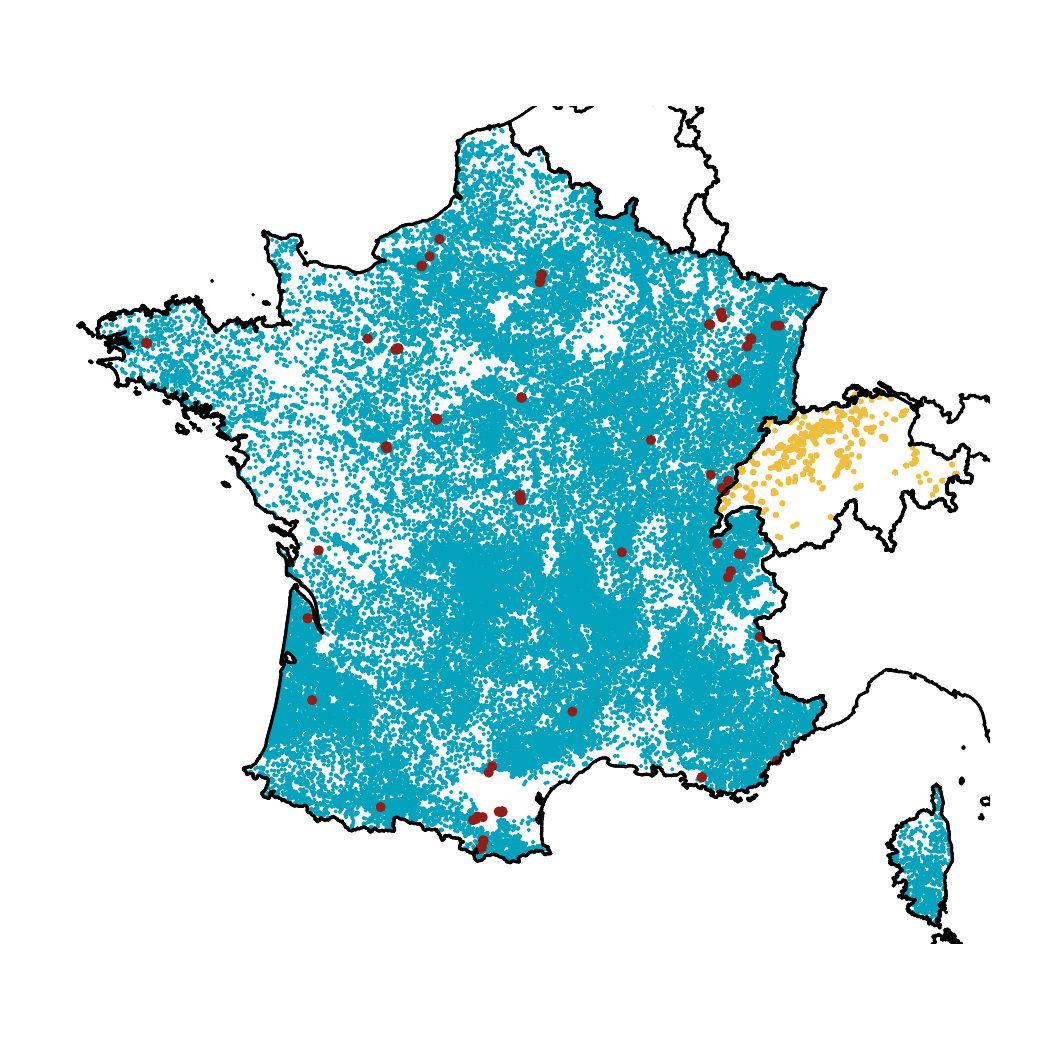
\includegraphics[width=\marginparwidth]{./Figures/map.png}
	\caption{Plot location for French \NFI, Emerge, and Swiss dataset.\label{fig::map}}
\end{marginfigure}

\begin{enumerate}
	\item `Protocole Oudin', dataset preserved by INRAE, ranging from 1930 to 1980 (in red on Fig. \ref{fig::map}). Recorded the bole volume, and the large and small branches. Hereafter, we name this dataset `Emerge', which was the name of the project that digitalised this dataset in 2008 \parencite{Deleuze2013}.
	\item The French \NFI (in blue on the Fig. \ref{fig::map}). Data range from 1988 to 2007 (data before 1988 record diameter rather than circumference). Recorded the bole volume.
	\item Experimental Forest Management project dataset \parencite[in yello on Fig. \ref{fig::map}]{Didion2024}. Data range from 1888 to 1974, and bole volume, large branches, and small branches were recorded.
	\item The `Office National des Forêts (ONF)', with protocols from 1972 and from 1983 (not used as there is no coordinates)
	\item Institut Technologique Forêt, Cellulose, Bois-construction, Ameublement (FCBA), not used so far for the aerial volume
	\item L'Institut pour le développement forestier (IDF) which is the R\&D of the Centre National de la Propriété Forestière and the Institut national de recherche en sciences et technologies pour l'environnement et l'agriculture (IRSTEA, currently INRAE)
\end{enumerate}

We decided to use the definitions from \cite{Gschwantner2009} (see Figs. \ref{fig::partition} and \ref{fig::ign_tree}):

\begin{marginfigure}%
	\begin{tikzpicture}
	\node (tree) at (0, 0) {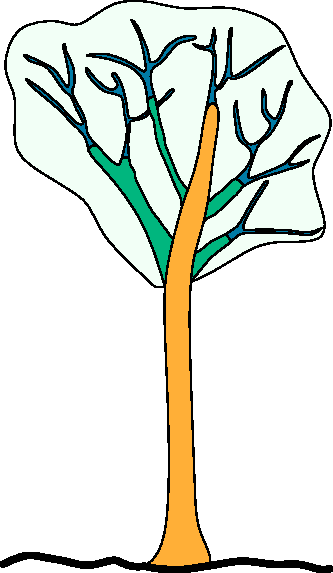
\includegraphics[width=\marginparwidth]{./Figures/ign_tree.pdf}};
	\matrix[below = -0.2cm of tree] {
		\node [draw, shape = rectangle, fill = egyptYellow, label = right:Bole] {}; \\
		\node [draw, shape = rectangle, fill = egyptGreen, label = right:Large branches] {}; \\
		\node [draw, shape = rectangle, fill = egyptBlue, label = right:Small branches] {}; \\
	};
\end{tikzpicture}
	\caption{Scheme of tree components.\label{fig::ign_tree}}
\end{marginfigure}

\begin{itemize}
	\item Main stem: The stem of a tree is the above-ground part of the main (off) shoot with apical dominance
	\begin{itemize}
		\item Stem top: topmost part of the stem from an over-bark base-diameter of \qty{7}{\centi\metre} (French \NFI) to the stem tip
		\item Bole: above-ground part of the stem between stump and the stem top
		\item Stump: above-ground base part of the stem which would remain after a tree was cut under normal felling practices
	\end{itemize}
	\item Lateral parts:
	\begin{itemize}
		\item Large branches: portion of the above-ground lateral parts with a diameter of more than or equal to \qty{7}{\centi\metre} (French \NFI)
		\item Large branches: portion of the above-ground lateral parts with a diameter of less than \qty{7}{\centi\metre} (French \NFI)
	\end{itemize}
\end{itemize}

A total of \num{594616} individuals were measured, with 98\% coming from the \NFI{} (bole volume only), 6\% from the Swiss dataset (bole, large and small branches), and 2\% from Emerge (same components as the Swiss dataset; see Fig. \ref{fig::compo}). The difficulties in fitting the data are twofold: first, the data show high heteroskedasticity (see Fig \ref{fig::fagSyl}), and second, the datasets are unbalanced.

\begin{figure}
	\centering
	% Created by tikzDevice version 0.12.6 on 2025-10-06 15:09:30
% !TEX encoding = UTF-8 Unicode
\begin{tikzpicture}[x=1pt,y=1pt,scale=0.6]
\definecolor{fillColor}{RGB}{255,255,255}
\path[use as bounding box,fill=fillColor,fill opacity=0.00] (0,0) rectangle (216.81,216.81);
\begin{scope}
\path[clip] (  0.00,  0.00) rectangle (216.81,216.81);
\definecolor{drawColor}{RGB}{0,0,0}
\definecolor{fillColor}{RGB}{147,30,24}

\path[draw=drawColor,line width= 0.4pt,line join=round,line cap=round,fill=fillColor] ( 60.00, 64.92) rectangle ( 63.54,101.09);
\definecolor{fillColor}{RGB}{240,190,61}

\path[draw=drawColor,line width= 0.4pt,line join=round,line cap=round,fill=fillColor] ( 60.00,108.32) rectangle (101.25,144.49);
\definecolor{fillColor}{RGB}{4,163,189}

\path[draw=drawColor,line width= 0.4pt,line join=round,line cap=round,fill=fillColor] ( 60.00,151.72) rectangle (192.81,187.89);
\end{scope}
\begin{scope}
\path[clip] (  0.00,  0.00) rectangle (216.81,216.81);
\definecolor{drawColor}{RGB}{0,0,0}

\node[text=drawColor,anchor=base east,inner sep=0pt, outer sep=0pt, scale=  0.75] at ( 48.00, 79.56) {Emerge};

\node[text=drawColor,anchor=base east,inner sep=0pt, outer sep=0pt, scale=  0.75] at ( 48.00,122.96) {\EFM};

\node[text=drawColor,anchor=base east,inner sep=0pt, outer sep=0pt, scale=  0.75] at ( 48.00,166.36) {\NFI};
\end{scope}
\begin{scope}
\path[clip] (  0.00,  0.00) rectangle (216.81,216.81);
\definecolor{drawColor}{RGB}{0,0,0}

\node[text=drawColor,anchor=base,inner sep=0pt, outer sep=0pt, scale=  0.75] at (126.41, 14.40) {Number of individuals};
\end{scope}
\begin{scope}
\path[clip] (  0.00,  0.00) rectangle (216.81,216.81);
\definecolor{drawColor}{RGB}{0,0,0}

\path[draw=drawColor,line width= 0.4pt,line join=round,line cap=round] ( 58.25, 60.00) -- (189.79, 60.00);

\path[draw=drawColor,line width= 0.4pt,line join=round,line cap=round] ( 58.25, 60.00) -- ( 58.25, 54.00);

\path[draw=drawColor,line width= 0.4pt,line join=round,line cap=round] ( 81.56, 60.00) -- ( 81.56, 54.00);

\path[draw=drawColor,line width= 0.4pt,line join=round,line cap=round] (112.37, 60.00) -- (112.37, 54.00);

\path[draw=drawColor,line width= 0.4pt,line join=round,line cap=round] (135.67, 60.00) -- (135.67, 54.00);

\path[draw=drawColor,line width= 0.4pt,line join=round,line cap=round] (158.98, 60.00) -- (158.98, 54.00);

\path[draw=drawColor,line width= 0.4pt,line join=round,line cap=round] (189.79, 60.00) -- (189.79, 54.00);

\node[text=drawColor,anchor=base,inner sep=0pt, outer sep=0pt, scale=  0.75] at ( 58.25, 38.40) {1e+04};

\node[text=drawColor,anchor=base,inner sep=0pt, outer sep=0pt, scale=  0.75] at (112.37, 38.40) {};

\node[text=drawColor,anchor=base,inner sep=0pt, outer sep=0pt, scale=  0.75] at (158.98, 38.40) {2e+05};
\end{scope}
\end{tikzpicture}

	\caption{Composition of the used dataset for the bole volume and total aerial volume.\label{fig::compo}}
\end{figure}

\begin{figure}
	\centering
	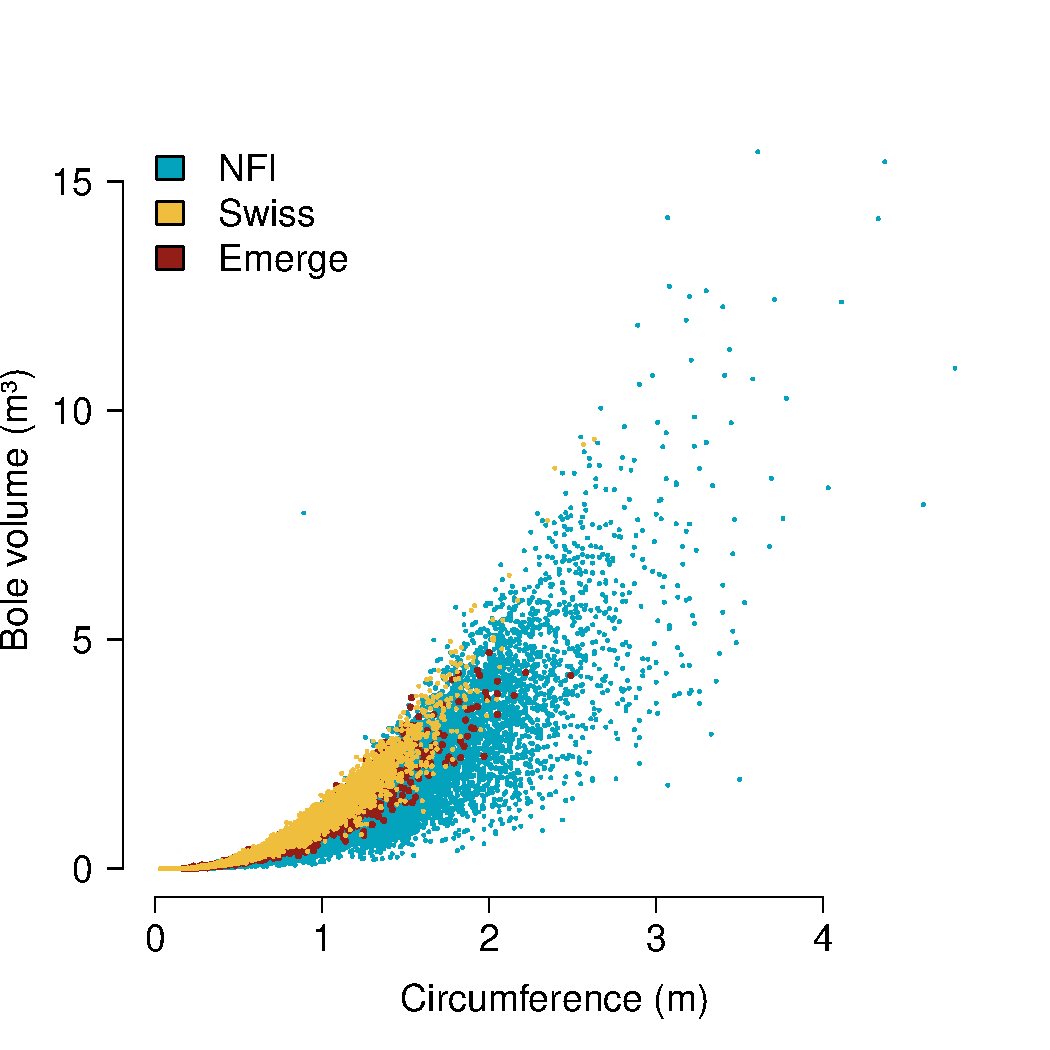
\includegraphics[scale = 0.5]{Figures/resp_fagus.pdf}
	\caption{Typical response of bole volume to circumference (here displayed for \textit{Fagus sylvatica}). We can see that both the Emerge and Swiss datasets \parencite{Deleuze2013,Didion2024} are quite similar and covers elongated trees, while the French \NFI{} covers less regular trees. \label{fig::fagSyl}}
\end{figure}

\begin{tcolorbox}[breakable, title = Bole volume (volume bois-fort tige)]
	The bole volume is the `reference' volume since the creation of the French \NFI{} (1958). Its definition is largely driven by the requirements of the wood industry, for which the estimation of standing timber volume is an essential tool for resource management and planning.
\end{tcolorbox}
\chapter{Bole volume\label{chap::bole_v}}
\begin{marginfigure}
	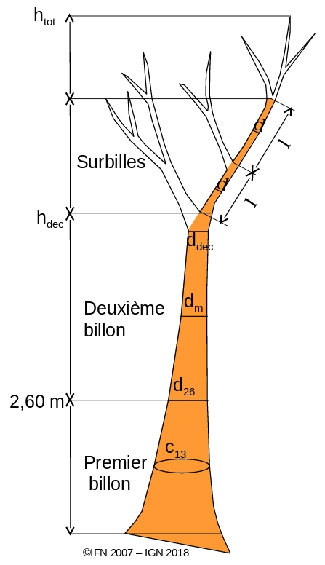
\includegraphics[width = \marginparwidth]{Figures/tree2.pdf}
	\caption{\label{fig::Vbole}}
\end{marginfigure}
The bole volume is considered the reference volume of the French \NFI{} and is computed via species-specific allometries. The formul\ae{} have changed over time, the most recent dating from 2016 \parencite{Morneau2016}. The allometric equations were fitted on the \NFI{} dataset, which contains the volumes of the butt log (from the stump to \qty{2.6}{\metre}), the second log (from \qty{2.6}{\metre} to \( \hdec \) --- defined in Tab. \ref{tab::notations}), and upper log sections if any (see Fig. \ref{fig::Vbole}). These three volumes rely on the circumferences at breast height, \qty{2.6}{\metre}, \( \hdec \), \( \ddec \), and the median diameter of the second log \( d_m \) and are derived using cylinder and Newton-Simpsons formul\ae{} \parencite{Gohon2024}. \\

In what follows, we sum up the equations currently used in the ``\nameref{sec::old_allom}'' section and compare them with new allometries recently developed \parencite{Gohon2024} in the section \nameref{sec::new_allom}. All the notations and definitions are gathered in Tab. \ref{tab::notations}.

\section{Two sets of equations\label{sec::old_allom}}

The annual living tree sample surveyed by the French \NFI{} is divided into two subsets:
\begin{description}
	\item [Complete trees] where girth (at breast height), \( c \), total height, \( h \), and taper height, \( \hdec \), are measured. These trees are randomly designated, ensuring that there is at least one individual per girth class, per species, and per plot.
	\item [Simplified trees] where only girth is measured.
\end{description}

For the so-called `complete trees', the bole volume is predicted using an allometric equation with three input variables (see equation \eqref{eq::fnew}), as described in \cite{Morneau2016}:
\begin{fullwidth}
	\begin{equation}
		\left\{
		\begin{aligned}
			\hat{V}_{\text{bole}} &= \frac{c^2 h}{4 \pi \left( 1 - \frac{1{,}3}{h} \right)^2} \hat f_{\text{new}} \\
			\hat f_{\text{new}} &= \left( \alpha + \beta c + \gamma \frac{\sqrt{c}}{h} + f(\hdec) + \delta \frac{1}{c^\epsilon} \right) \left[ 1 - b \left( \frac{0{,}07 \pi}{c} \right)^3 \left( 1 - \frac{1{,}3}{h} \right)^3 \right],
		\end{aligned}
		\right.
		\label{eq::fnew}
	\end{equation}
\end{fullwidth}
where \( f \) is a function of \( \hdec \) among the following:
\begin{alignat*}{2}
f(\hdec) & = f_{\text{max}}\!\left( \frac{\hdec}{\hdec + k} \right)^{1 + \rho} && \qquad f(\hdec) = \eta \ln\!\left( \frac{\hdec}{h} \right) \\
f(\hdec) & = \eta \ln(\hdec) && \qquad f(\hdec) = \eta \hdec
\end{alignat*}
The coefficients \( \alpha \) \dots, \( b \), and the function \( f \) are species-specific. Some of these coefficients also depend on the kind of terminal cut of the tree, either the stem top (\textit{regular cut}) or a sudden decrease in stem diameter (\textit{shape cut}). \\

For simplified trees, the bole volume is based on the predicted volume of a neighbouring complete tree. A one-variable allometric equation is used to adjust for the girth difference between the reference tree and the simplified tree when assigning bole volume.
\begin{tcolorbox}[breakable, title = Volume imputation]
We associate each simplified tree \( i \) with a complete tree \( j \) that belongs to the same plot, same species and same girth class and adjust the bole volume of \( i \) using a ratio relative to its reference tree:
	\begin{equation}
		\hat{V}_{\text{bole}}^{\text{imp}}(i) = \hat{V}_{\text{bole}}(j) \frac{V_{I}(i)}{V_{I}(j)},
		\label{eq::imputation}
	\end{equation}
	where \( \hat{V}_{\text{bole}} \) is the three variable equation \eqref{eq::fnew}, and \( V_{I} \) is a species-specific allometric equation that takes only \( c \) as an input variable (see equation \eqref{eq::allom_1}).
\end{tcolorbox}

Current one-variable allometric equations are built on log transformation:
\begin{fullwidth}
	\begin{equation}
		V_{I} = \exp \left[ \alpha + \beta \ln(c) + \gamma \ln(c)^2 + \delta \ln(c)^3 + \zeta \ln(c)^4 + \eta f(g) + \frac{\sigma^2}{2} \right],
		\label{eq::allom_1}
	\end{equation}
\end{fullwidth}
where \( f(g) \) is a function of local basal area. The coefficients \( \alpha \), \dots, \( \sigma \) depend on the tree species and contextual parameters (ecological area, altitude zone, property regime). 

\section{Motivations for changes}

Regarding the three-variable allometric equations (Eq. \eqref{eq::fnew}), the aim is to improve model parsimony so that future species models share the same formula and fitting no longer depends on the type of terminal cut. Also, a decision was made to no longer rely on the \( \hdec \) term for trees with regular cuts, since \( \hdec \) has not been measured for such trees since 2020 and must now be estimated using a third-party model. This is achieved by defining \( \hdec' \) as:
\[
	\hdec' =
	\begin{cases}
		\hdec & \text{in case of a shape cut} \\
		h & \text{otherwise}
	\end{cases}
\]

For monitoring stock variations over time, the new coming inventory method will assess tree sample data twice. Tree samples are surveyed a second time, but only tree girth is measured again. So, one-variable allometric equations shall be used to assess tree new volume at second survey given old and new girth, the same way than simplified trees (see \ref{eq::imputation}). For that purpose, one-variable volume equations have to be an increasing function of girth. In particular, an explanatory variable \( f(g) \) involving local basal area, conveying stand competition, has to be questioned.  

The approach of new allometric equations development is detailed in \cite{Gohon2024}.  

\section{New bole models\label{sec::new_allom}}

Like current equations, future three-variable models are fitted using French NFI data (see \ref{chap::def} 3.). It models a shape coefficient \( f_{\text{new}} \) (see \ref{eq::fnew}) an analogous way than \cite{Morneau2016}.  

\[
	\hat f_{\text{new}} = \alpha + \beta c + \gamma \frac{\sqrt{c}}{\hdec'} + \delta \frac{\sqrt{\hdec'}}{c^2 h} + \eta \left( 1 - \frac{\hdec'}{h} \right)
\]
where coefficients (\( \alpha \), \( \beta \), \( \gamma \), \( \delta \), \( \eta \)) only depend on the tree species.  

New single-variable models are fitted to volume estimates of complete trees from recent inventory campaigns.

\[
	V_{I} = \mathrm{e}^{\alpha + \beta \ln(c) + \gamma \ln(c)^2 + \frac{\sigma^2}{2}},
\]
where (\( \alpha \), \( \beta \), \( \gamma \), \( \sigma \)) still depend on the tree species and on the same contextual parameters (ecological area, altitude zone, property regime).

New and current models perform similarly.
Survey estimates (see for instance \ref{fig::estimate_vbole_bygirth} and \ref{fig::estimate_vbole} from \cite{Gohon2024}) are a go-to output to foresee the forthcoming effect of new allometric equations on \NFI{} results. It shows lower volume estimates for small trees and slightly higher volume estimates for bigger trees, and consequently higher volume growth estimates. Differences never exceed confidence intervals.

\begin{figure}[h]
	\centering
	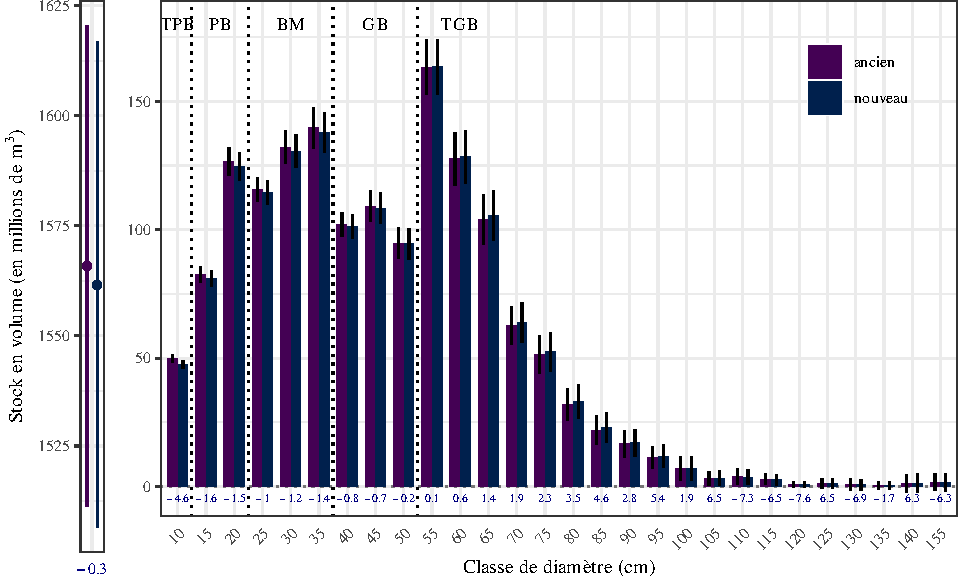
\includegraphics[scale = 0.6]{Figures/estimate_vbole_bygirth.pdf}
	\caption{National bole volume estimates for trees with height measures, by rounded girth. \label{fig::estimate_vbole_bygirth}}
\end{figure}

\begin{figure}[h]
	\centering
	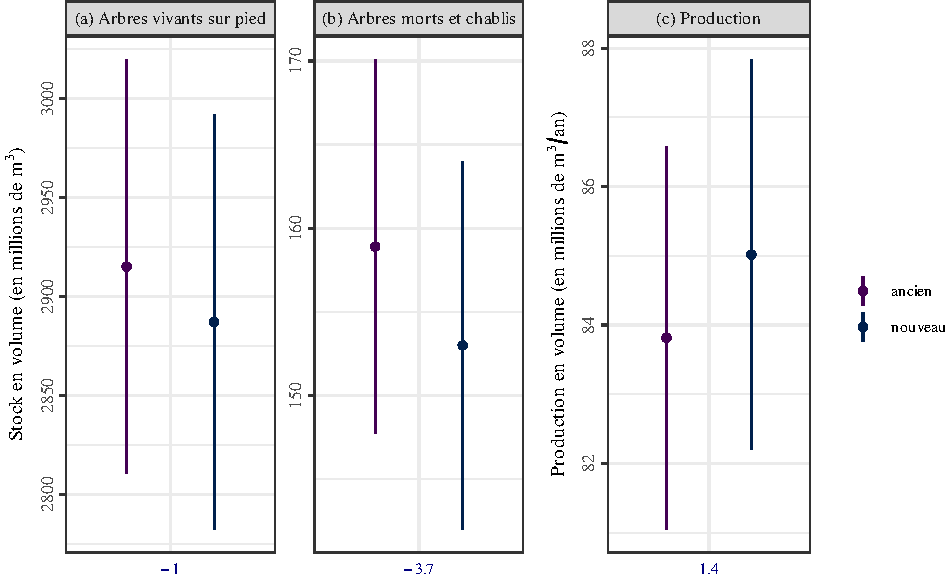
\includegraphics[scale = 0.6]{Figures/estimate_vbole.pdf}
	\caption{National bole volume and growth estimates for all living trees and dead trees. \label{fig::estimate_vbole}}
\end{figure}

\chapter{Total aerial volume\label{chap::total_v}}

In this section, I explore two possible paths to estimate the total aerial volume, \( \Vtot \). The first option, based on \cite{Longuetaud2013}, uses the ratio:
\begin{equation}
	r = \frac{\Vbole}{\Vtot} \label{eq::r_boletot}
\end{equation}
and is comprised between 0 and 1 by construction. Therefore, a Beta-distribution is a good fit. The second option is to fit a multivariate normal distribution, \( \MVN \), to the \textit{transformed} ratio, \( \logit(r) \), jointly with the log-transformed total volume, \( \log(\Vtot) \):
\begin{equation}
	\begin{pmatrix}
		\logit(r) \\
		\log(\Vtot)
	\end{pmatrix}
	\sim
	\MVN\left\{ \begin{pmatrix}
		f(c, \, h; \symbfup{\theta}) \\
		g(c, \, h; \symbfup{\theta}) \\
	\end{pmatrix}, \symbfup{\Sigma} \right\},
	\label{eq::mvn}
\end{equation}
where \( f \) and \( g \) are functions to tailor for our specific needs, \( c \) is circumference at breast height, \( h \), is tree height, and \( \theta \) is a vector of parameters to estimate.

\section{Ratio approach}

\section{Multivariate approach}

\subsection{Simulated data}
In order to demonstrate the relevance of multivariate methods, I simulate two correlated random variables and then recover the generating parameters.

\printbibliography

\end{document}
